\documentclass[twoside]{book}

% Packages required by doxygen
\usepackage{fixltx2e}
\usepackage{calc}
\usepackage{doxygen}
\usepackage[export]{adjustbox} % also loads graphicx
\usepackage{graphicx}
\usepackage[utf8]{inputenc}
\usepackage{makeidx}
\usepackage{multicol}
\usepackage{multirow}
\PassOptionsToPackage{warn}{textcomp}
\usepackage{textcomp}
\usepackage[nointegrals]{wasysym}
\usepackage[table]{xcolor}

% Font selection
\usepackage[T1]{fontenc}
\usepackage[scaled=.90]{helvet}
\usepackage{courier}
\usepackage{amssymb}
\usepackage{sectsty}
\renewcommand{\familydefault}{\sfdefault}
\allsectionsfont{%
  \fontseries{bc}\selectfont%
  \color{darkgray}%
}
\renewcommand{\DoxyLabelFont}{%
  \fontseries{bc}\selectfont%
  \color{darkgray}%
}
\newcommand{\+}{\discretionary{\mbox{\scriptsize$\hookleftarrow$}}{}{}}

% Page & text layout
\usepackage{geometry}
\geometry{%
  a4paper,%
  top=2.5cm,%
  bottom=2.5cm,%
  left=2.5cm,%
  right=2.5cm%
}
\tolerance=750
\hfuzz=15pt
\hbadness=750
\setlength{\emergencystretch}{15pt}
\setlength{\parindent}{0cm}
\setlength{\parskip}{3ex plus 2ex minus 2ex}
\makeatletter
\renewcommand{\paragraph}{%
  \@startsection{paragraph}{4}{0ex}{-1.0ex}{1.0ex}{%
    \normalfont\normalsize\bfseries\SS@parafont%
  }%
}
\renewcommand{\subparagraph}{%
  \@startsection{subparagraph}{5}{0ex}{-1.0ex}{1.0ex}{%
    \normalfont\normalsize\bfseries\SS@subparafont%
  }%
}
\makeatother

% Headers & footers
\usepackage{fancyhdr}
\pagestyle{fancyplain}
\fancyhead[LE]{\fancyplain{}{\bfseries\thepage}}
\fancyhead[CE]{\fancyplain{}{}}
\fancyhead[RE]{\fancyplain{}{\bfseries\leftmark}}
\fancyhead[LO]{\fancyplain{}{\bfseries\rightmark}}
\fancyhead[CO]{\fancyplain{}{}}
\fancyhead[RO]{\fancyplain{}{\bfseries\thepage}}
\fancyfoot[LE]{\fancyplain{}{}}
\fancyfoot[CE]{\fancyplain{}{}}
\fancyfoot[RE]{\fancyplain{}{\bfseries\scriptsize Generated by Doxygen }}
\fancyfoot[LO]{\fancyplain{}{\bfseries\scriptsize Generated by Doxygen }}
\fancyfoot[CO]{\fancyplain{}{}}
\fancyfoot[RO]{\fancyplain{}{}}
\renewcommand{\footrulewidth}{0.4pt}
\renewcommand{\chaptermark}[1]{%
  \markboth{#1}{}%
}
\renewcommand{\sectionmark}[1]{%
  \markright{\thesection\ #1}%
}

% Indices & bibliography
\usepackage{natbib}
\usepackage[titles]{tocloft}
\setcounter{tocdepth}{3}
\setcounter{secnumdepth}{5}
\makeindex

% Hyperlinks (required, but should be loaded last)
\usepackage{ifpdf}
\ifpdf
  \usepackage[pdftex,pagebackref=true]{hyperref}
\else
  \usepackage[ps2pdf,pagebackref=true]{hyperref}
\fi
\hypersetup{%
  colorlinks=true,%
  linkcolor=blue,%
  citecolor=blue,%
  unicode%
}

% Custom commands
\newcommand{\clearemptydoublepage}{%
  \newpage{\pagestyle{empty}\cleardoublepage}%
}

\usepackage{caption}
\captionsetup{labelsep=space,justification=centering,font={bf},singlelinecheck=off,skip=4pt,position=top}

%===== C O N T E N T S =====

\begin{document}

% Titlepage & ToC
\hypersetup{pageanchor=false,
             bookmarksnumbered=true,
             pdfencoding=unicode
            }
\pagenumbering{roman}
\begin{titlepage}
\vspace*{7cm}
\begin{center}%
{\Large My Project }\\
\vspace*{1cm}
{\large Generated by Doxygen 1.8.11}\\
\end{center}
\end{titlepage}
\clearemptydoublepage
\tableofcontents
\clearemptydoublepage
\pagenumbering{arabic}
\hypersetup{pageanchor=true}

%--- Begin generated contents ---
\chapter{Class Index}
\section{Class List}
Here are the classes, structs, unions and interfaces with brief descriptions\+:\begin{DoxyCompactList}
\item\contentsline{section}{\hyperlink{structnode}{node} }{\pageref{structnode}}{}
\item\contentsline{section}{\hyperlink{structnode1}{node1} }{\pageref{structnode1}}{}
\item\contentsline{section}{\hyperlink{structnode__info}{node\+\_\+info} }{\pageref{structnode__info}}{}
\end{DoxyCompactList}

\chapter{File Index}
\section{File List}
Here is a list of all files with brief descriptions\+:\begin{DoxyCompactList}
\item\contentsline{section}{\hyperlink{Lab1_8c}{Lab1.\+c} }{\pageref{Lab1_8c}}{}
\end{DoxyCompactList}

\chapter{Class Documentation}
\hypertarget{classAc}{}\section{Ac Class Reference}
\label{classAc}\index{Ac@{Ac}}
\subsection*{Public Member Functions}
\begin{DoxyCompactItemize}
\item 
void \hyperlink{classAc_a0962ee2f69390f3ed8f44dd97c9f859a}{ac\+On} ()
\item 
void \hyperlink{classAc_ac6c08e83b03e986786f9de290c55bcf0}{ac\+Off} ()
\end{DoxyCompactItemize}


\subsection{Member Function Documentation}
\index{Ac@{Ac}!ac\+Off@{ac\+Off}}
\index{ac\+Off@{ac\+Off}!Ac@{Ac}}
\subsubsection[{\texorpdfstring{ac\+Off()}{acOff()}}]{\setlength{\rightskip}{0pt plus 5cm}void Ac\+::ac\+Off (
\begin{DoxyParamCaption}
{}
\end{DoxyParamCaption}
)\hspace{0.3cm}{\ttfamily [inline]}}\hypertarget{classAc_ac6c08e83b03e986786f9de290c55bcf0}{}\label{classAc_ac6c08e83b03e986786f9de290c55bcf0}

\begin{DoxyCode}
40     \{
41         cout << \textcolor{stringliteral}{"AC is off"}<<endl;
42     \}
\end{DoxyCode}
\index{Ac@{Ac}!ac\+On@{ac\+On}}
\index{ac\+On@{ac\+On}!Ac@{Ac}}
\subsubsection[{\texorpdfstring{ac\+On()}{acOn()}}]{\setlength{\rightskip}{0pt plus 5cm}void Ac\+::ac\+On (
\begin{DoxyParamCaption}
{}
\end{DoxyParamCaption}
)\hspace{0.3cm}{\ttfamily [inline]}}\hypertarget{classAc_a0962ee2f69390f3ed8f44dd97c9f859a}{}\label{classAc_a0962ee2f69390f3ed8f44dd97c9f859a}

\begin{DoxyCode}
35     \{
36         cout << \textcolor{stringliteral}{"Ac is on"}<<endl;
37     \}
\end{DoxyCode}


The documentation for this class was generated from the following file\+:\begin{DoxyCompactItemize}
\item 
\hyperlink{Facade_8cpp}{Facade.\+cpp}\end{DoxyCompactItemize}

\hypertarget{classAlarm}{}\section{Alarm Class Reference}
\label{classAlarm}\index{Alarm@{Alarm}}
\subsection*{Public Member Functions}
\begin{DoxyCompactItemize}
\item 
void \hyperlink{classAlarm_a1887c06d8efdf5b4805314a6eac48098}{alarm\+On} ()
\item 
void \hyperlink{classAlarm_a53104c545f8e12865c049854379e32d7}{alarm\+Off} ()
\end{DoxyCompactItemize}


\subsection{Member Function Documentation}
\index{Alarm@{Alarm}!alarm\+Off@{alarm\+Off}}
\index{alarm\+Off@{alarm\+Off}!Alarm@{Alarm}}
\subsubsection[{\texorpdfstring{alarm\+Off()}{alarmOff()}}]{\setlength{\rightskip}{0pt plus 5cm}void Alarm\+::alarm\+Off (
\begin{DoxyParamCaption}
{}
\end{DoxyParamCaption}
)\hspace{0.3cm}{\ttfamily [inline]}}\hypertarget{classAlarm_a53104c545f8e12865c049854379e32d7}{}\label{classAlarm_a53104c545f8e12865c049854379e32d7}

\begin{DoxyCode}
26     \{
27         cout << \textcolor{stringliteral}{"Alarm is off and you can go into the house"}<<endl;
28     \}
\end{DoxyCode}
\index{Alarm@{Alarm}!alarm\+On@{alarm\+On}}
\index{alarm\+On@{alarm\+On}!Alarm@{Alarm}}
\subsubsection[{\texorpdfstring{alarm\+On()}{alarmOn()}}]{\setlength{\rightskip}{0pt plus 5cm}void Alarm\+::alarm\+On (
\begin{DoxyParamCaption}
{}
\end{DoxyParamCaption}
)\hspace{0.3cm}{\ttfamily [inline]}}\hypertarget{classAlarm_a1887c06d8efdf5b4805314a6eac48098}{}\label{classAlarm_a1887c06d8efdf5b4805314a6eac48098}

\begin{DoxyCode}
21     \{
22         cout << \textcolor{stringliteral}{"Alarm is on and house is secured"}<<endl;
23     \}
\end{DoxyCode}


The documentation for this class was generated from the following file\+:\begin{DoxyCompactItemize}
\item 
\hyperlink{Facade_8cpp}{Facade.\+cpp}\end{DoxyCompactItemize}

\hypertarget{classHouseFacade}{}\section{House\+Facade Class Reference}
\label{classHouseFacade}\index{House\+Facade@{House\+Facade}}


Collaboration diagram for House\+Facade\+:
\nopagebreak
\begin{figure}[H]
\begin{center}
\leavevmode
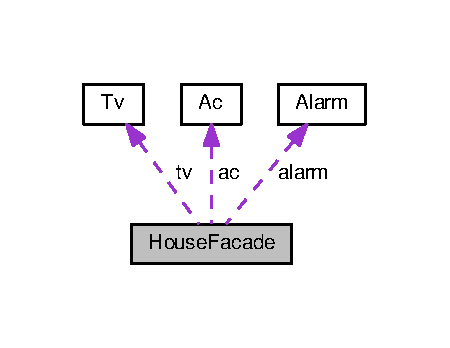
\includegraphics[width=216pt]{classHouseFacade__coll__graph}
\end{center}
\end{figure}
\subsection*{Public Member Functions}
\begin{DoxyCompactItemize}
\item 
\hyperlink{classHouseFacade_abab7c9304c5123ad2894a86d071a4e51}{House\+Facade} ()
\item 
void \hyperlink{classHouseFacade_af62723fc617325d0ea4918349cb66dbb}{go\+To\+Work} ()
\item 
void \hyperlink{classHouseFacade_a806337202c3a039456a180777d034684}{come\+Home} ()
\end{DoxyCompactItemize}
\subsection*{Private Attributes}
\begin{DoxyCompactItemize}
\item 
\hyperlink{classAlarm}{Alarm} \hyperlink{classHouseFacade_a9635b0a634d8fc7be556c9dd33782cb9}{alarm}
\item 
\hyperlink{classAc}{Ac} \hyperlink{classHouseFacade_a6d30f8878c9f220d37f5866084466d35}{ac}
\item 
\hyperlink{classTv}{Tv} \hyperlink{classHouseFacade_a58d2375afc4bed9ae74bd18cf4dd79ef}{tv}
\end{DoxyCompactItemize}


\subsection{Constructor \& Destructor Documentation}
\index{House\+Facade@{House\+Facade}!House\+Facade@{House\+Facade}}
\index{House\+Facade@{House\+Facade}!House\+Facade@{House\+Facade}}
\subsubsection[{\texorpdfstring{House\+Facade()}{HouseFacade()}}]{\setlength{\rightskip}{0pt plus 5cm}House\+Facade\+::\+House\+Facade (
\begin{DoxyParamCaption}
{}
\end{DoxyParamCaption}
)\hspace{0.3cm}{\ttfamily [inline]}}\hypertarget{classHouseFacade_abab7c9304c5123ad2894a86d071a4e51}{}\label{classHouseFacade_abab7c9304c5123ad2894a86d071a4e51}

\begin{DoxyCode}
66 \{\}
\end{DoxyCode}


\subsection{Member Function Documentation}
\index{House\+Facade@{House\+Facade}!come\+Home@{come\+Home}}
\index{come\+Home@{come\+Home}!House\+Facade@{House\+Facade}}
\subsubsection[{\texorpdfstring{come\+Home()}{comeHome()}}]{\setlength{\rightskip}{0pt plus 5cm}void House\+Facade\+::come\+Home (
\begin{DoxyParamCaption}
{}
\end{DoxyParamCaption}
)\hspace{0.3cm}{\ttfamily [inline]}}\hypertarget{classHouseFacade_a806337202c3a039456a180777d034684}{}\label{classHouseFacade_a806337202c3a039456a180777d034684}

\begin{DoxyCode}
76     \{
77         \hyperlink{classHouseFacade_a9635b0a634d8fc7be556c9dd33782cb9}{alarm}.\hyperlink{classAlarm_a53104c545f8e12865c049854379e32d7}{alarmOff}();
78         \hyperlink{classHouseFacade_a6d30f8878c9f220d37f5866084466d35}{ac}.\hyperlink{classAc_a0962ee2f69390f3ed8f44dd97c9f859a}{acOn}();
79         \hyperlink{classHouseFacade_a58d2375afc4bed9ae74bd18cf4dd79ef}{tv}.\hyperlink{classTv_ad966c38bf07398f9b2a70ded516c2479}{tvOn}();
80     \}
\end{DoxyCode}


Here is the call graph for this function\+:
\nopagebreak
\begin{figure}[H]
\begin{center}
\leavevmode
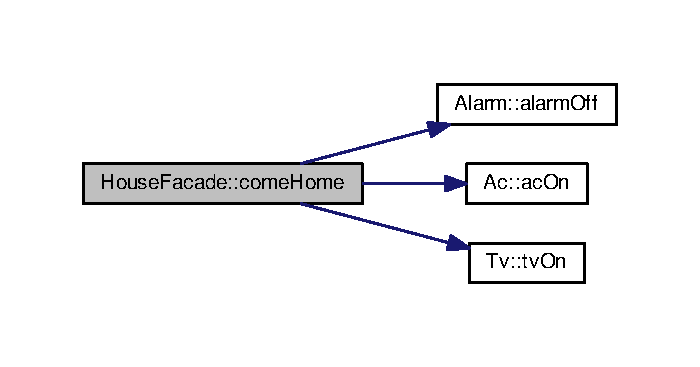
\includegraphics[width=336pt]{classHouseFacade_a806337202c3a039456a180777d034684_cgraph}
\end{center}
\end{figure}


\index{House\+Facade@{House\+Facade}!go\+To\+Work@{go\+To\+Work}}
\index{go\+To\+Work@{go\+To\+Work}!House\+Facade@{House\+Facade}}
\subsubsection[{\texorpdfstring{go\+To\+Work()}{goToWork()}}]{\setlength{\rightskip}{0pt plus 5cm}void House\+Facade\+::go\+To\+Work (
\begin{DoxyParamCaption}
{}
\end{DoxyParamCaption}
)\hspace{0.3cm}{\ttfamily [inline]}}\hypertarget{classHouseFacade_af62723fc617325d0ea4918349cb66dbb}{}\label{classHouseFacade_af62723fc617325d0ea4918349cb66dbb}

\begin{DoxyCode}
69     \{
70         \hyperlink{classHouseFacade_a6d30f8878c9f220d37f5866084466d35}{ac}.\hyperlink{classAc_ac6c08e83b03e986786f9de290c55bcf0}{acOff}();
71         \hyperlink{classHouseFacade_a58d2375afc4bed9ae74bd18cf4dd79ef}{tv}.\hyperlink{classTv_a407913fbb5490cb137cf89b9932497d0}{tvOff}();
72         \hyperlink{classHouseFacade_a9635b0a634d8fc7be556c9dd33782cb9}{alarm}.\hyperlink{classAlarm_a1887c06d8efdf5b4805314a6eac48098}{alarmOn}();
73     \}
\end{DoxyCode}


Here is the call graph for this function\+:
\nopagebreak
\begin{figure}[H]
\begin{center}
\leavevmode
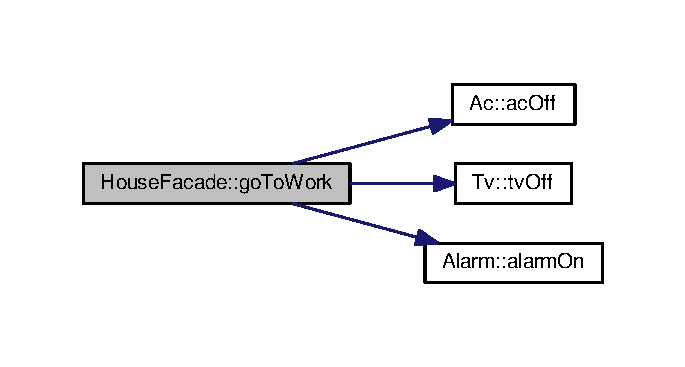
\includegraphics[width=329pt]{classHouseFacade_af62723fc617325d0ea4918349cb66dbb_cgraph}
\end{center}
\end{figure}




\subsection{Member Data Documentation}
\index{House\+Facade@{House\+Facade}!ac@{ac}}
\index{ac@{ac}!House\+Facade@{House\+Facade}}
\subsubsection[{\texorpdfstring{ac}{ac}}]{\setlength{\rightskip}{0pt plus 5cm}{\bf Ac} House\+Facade\+::ac\hspace{0.3cm}{\ttfamily [private]}}\hypertarget{classHouseFacade_a6d30f8878c9f220d37f5866084466d35}{}\label{classHouseFacade_a6d30f8878c9f220d37f5866084466d35}
\index{House\+Facade@{House\+Facade}!alarm@{alarm}}
\index{alarm@{alarm}!House\+Facade@{House\+Facade}}
\subsubsection[{\texorpdfstring{alarm}{alarm}}]{\setlength{\rightskip}{0pt plus 5cm}{\bf Alarm} House\+Facade\+::alarm\hspace{0.3cm}{\ttfamily [private]}}\hypertarget{classHouseFacade_a9635b0a634d8fc7be556c9dd33782cb9}{}\label{classHouseFacade_a9635b0a634d8fc7be556c9dd33782cb9}
\index{House\+Facade@{House\+Facade}!tv@{tv}}
\index{tv@{tv}!House\+Facade@{House\+Facade}}
\subsubsection[{\texorpdfstring{tv}{tv}}]{\setlength{\rightskip}{0pt plus 5cm}{\bf Tv} House\+Facade\+::tv\hspace{0.3cm}{\ttfamily [private]}}\hypertarget{classHouseFacade_a58d2375afc4bed9ae74bd18cf4dd79ef}{}\label{classHouseFacade_a58d2375afc4bed9ae74bd18cf4dd79ef}


The documentation for this class was generated from the following file\+:\begin{DoxyCompactItemize}
\item 
\hyperlink{Facade_8cpp}{Facade.\+cpp}\end{DoxyCompactItemize}

\hypertarget{classTv}{}\section{Tv Class Reference}
\label{classTv}\index{Tv@{Tv}}
\subsection*{Public Member Functions}
\begin{DoxyCompactItemize}
\item 
void \hyperlink{classTv_ad966c38bf07398f9b2a70ded516c2479}{tv\+On} ()
\item 
void \hyperlink{classTv_a407913fbb5490cb137cf89b9932497d0}{tv\+Off} ()
\end{DoxyCompactItemize}


\subsection{Member Function Documentation}
\index{Tv@{Tv}!tv\+Off@{tv\+Off}}
\index{tv\+Off@{tv\+Off}!Tv@{Tv}}
\subsubsection[{\texorpdfstring{tv\+Off()}{tvOff()}}]{\setlength{\rightskip}{0pt plus 5cm}void Tv\+::tv\+Off (
\begin{DoxyParamCaption}
{}
\end{DoxyParamCaption}
)\hspace{0.3cm}{\ttfamily [inline]}}\hypertarget{classTv_a407913fbb5490cb137cf89b9932497d0}{}\label{classTv_a407913fbb5490cb137cf89b9932497d0}

\begin{DoxyCode}
54     \{
55         cout << \textcolor{stringliteral}{"TV is off"}<<endl;
56     \}
\end{DoxyCode}
\index{Tv@{Tv}!tv\+On@{tv\+On}}
\index{tv\+On@{tv\+On}!Tv@{Tv}}
\subsubsection[{\texorpdfstring{tv\+On()}{tvOn()}}]{\setlength{\rightskip}{0pt plus 5cm}void Tv\+::tv\+On (
\begin{DoxyParamCaption}
{}
\end{DoxyParamCaption}
)\hspace{0.3cm}{\ttfamily [inline]}}\hypertarget{classTv_ad966c38bf07398f9b2a70ded516c2479}{}\label{classTv_ad966c38bf07398f9b2a70ded516c2479}

\begin{DoxyCode}
49     \{
50         cout << \textcolor{stringliteral}{"Tv is on"}<<endl;
51     \}
\end{DoxyCode}


The documentation for this class was generated from the following file\+:\begin{DoxyCompactItemize}
\item 
\hyperlink{Facade_8cpp}{Facade.\+cpp}\end{DoxyCompactItemize}

\chapter{File Documentation}
\hypertarget{Facade_8cpp}{}\section{Facade.\+cpp File Reference}
\label{Facade_8cpp}\index{Facade.\+cpp@{Facade.\+cpp}}
{\ttfamily \#include $<$string$>$}\\*
{\ttfamily \#include $<$iostream$>$}\\*
Include dependency graph for Facade.\+cpp\+:
\nopagebreak
\begin{figure}[H]
\begin{center}
\leavevmode
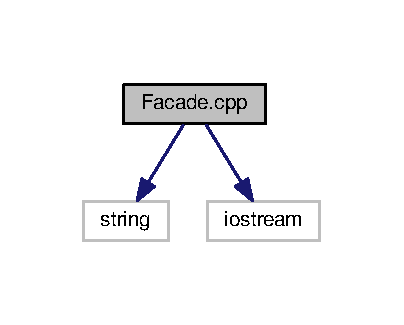
\includegraphics[width=194pt]{Facade_8cpp__incl}
\end{center}
\end{figure}
\subsection*{Classes}
\begin{DoxyCompactItemize}
\item 
class \hyperlink{classAlarm}{Alarm}
\item 
class \hyperlink{classAc}{Ac}
\item 
class \hyperlink{classTv}{Tv}
\item 
class \hyperlink{classHouseFacade}{House\+Facade}
\end{DoxyCompactItemize}
\subsection*{Functions}
\begin{DoxyCompactItemize}
\item 
int \hyperlink{Facade_8cpp_ae66f6b31b5ad750f1fe042a706a4e3d4}{main} ()
\end{DoxyCompactItemize}


\subsection{Function Documentation}
\index{Facade.\+cpp@{Facade.\+cpp}!main@{main}}
\index{main@{main}!Facade.\+cpp@{Facade.\+cpp}}
\subsubsection[{\texorpdfstring{main()}{main()}}]{\setlength{\rightskip}{0pt plus 5cm}int main (
\begin{DoxyParamCaption}
{}
\end{DoxyParamCaption}
)}\hypertarget{Facade_8cpp_ae66f6b31b5ad750f1fe042a706a4e3d4}{}\label{Facade_8cpp_ae66f6b31b5ad750f1fe042a706a4e3d4}

\begin{DoxyCode}
84 \{
85     \hyperlink{classHouseFacade}{HouseFacade} hf;
86 
87     \textcolor{comment}{//Rather than calling 100 different on and off functions thanks to facade I only have 2 functions...}
88     hf.\hyperlink{classHouseFacade_af62723fc617325d0ea4918349cb66dbb}{goToWork}();
89     hf.\hyperlink{classHouseFacade_a806337202c3a039456a180777d034684}{comeHome}();
90 \}\end{DoxyCode}


Here is the call graph for this function\+:
\nopagebreak
\begin{figure}[H]
\begin{center}
\leavevmode
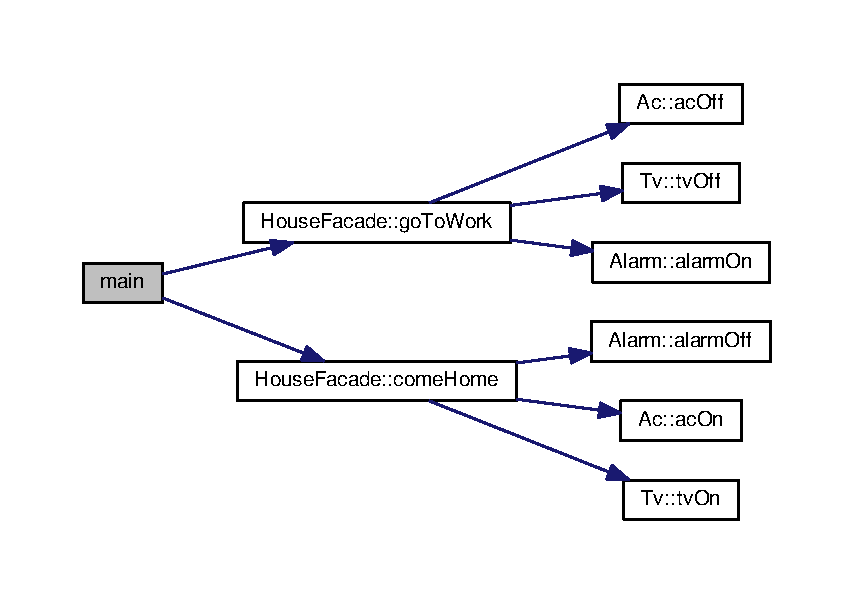
\includegraphics[width=350pt]{Facade_8cpp_ae66f6b31b5ad750f1fe042a706a4e3d4_cgraph}
\end{center}
\end{figure}



%--- End generated contents ---

% Index
\backmatter
\newpage
\phantomsection
\clearemptydoublepage
\addcontentsline{toc}{chapter}{Index}
\printindex

\end{document}
